% Options for packages loaded elsewhere
\PassOptionsToPackage{unicode}{hyperref}
\PassOptionsToPackage{hyphens}{url}
%
\documentclass[
  12pt,
]{article}
\usepackage{lmodern}
\usepackage{amssymb,amsmath}
\usepackage{ifxetex,ifluatex}
\ifnum 0\ifxetex 1\fi\ifluatex 1\fi=0 % if pdftex
  \usepackage[T1]{fontenc}
  \usepackage[utf8]{inputenc}
  \usepackage{textcomp} % provide euro and other symbols
\else % if luatex or xetex
  \usepackage{unicode-math}
  \defaultfontfeatures{Scale=MatchLowercase}
  \defaultfontfeatures[\rmfamily]{Ligatures=TeX,Scale=1}
  \setmainfont[]{Times New Roman}
\fi
% Use upquote if available, for straight quotes in verbatim environments
\IfFileExists{upquote.sty}{\usepackage{upquote}}{}
\IfFileExists{microtype.sty}{% use microtype if available
  \usepackage[]{microtype}
  \UseMicrotypeSet[protrusion]{basicmath} % disable protrusion for tt fonts
}{}
\makeatletter
\@ifundefined{KOMAClassName}{% if non-KOMA class
  \IfFileExists{parskip.sty}{%
    \usepackage{parskip}
  }{% else
    \setlength{\parindent}{0pt}
    \setlength{\parskip}{6pt plus 2pt minus 1pt}}
}{% if KOMA class
  \KOMAoptions{parskip=half}}
\makeatother
\usepackage{xcolor}
\IfFileExists{xurl.sty}{\usepackage{xurl}}{} % add URL line breaks if available
\IfFileExists{bookmark.sty}{\usepackage{bookmark}}{\usepackage{hyperref}}
\hypersetup{
  pdftitle={Estimating Carrying Capacity for Juvenile Salmon using Quantile Random Forest Models},
  pdfauthor={Kevin E. See1,, Michael W. Ackerman1, Richard A. Carmichael1, Sarah L. Hoffmann1, and Chris Beasley1},
  pdfkeywords={carrying capacity; Chinook salmon; quantile random forest; quantile regression; random forests},
  hidelinks,
  pdfcreator={LaTeX via pandoc}}
\urlstyle{same} % disable monospaced font for URLs
\usepackage[margin=1in]{geometry}
\usepackage{longtable,booktabs}
% Correct order of tables after \paragraph or \subparagraph
\usepackage{etoolbox}
\makeatletter
\patchcmd\longtable{\par}{\if@noskipsec\mbox{}\fi\par}{}{}
\makeatother
% Allow footnotes in longtable head/foot
\IfFileExists{footnotehyper.sty}{\usepackage{footnotehyper}}{\usepackage{footnote}}
\makesavenoteenv{longtable}
\usepackage{graphicx,grffile}
\makeatletter
\def\maxwidth{\ifdim\Gin@nat@width>\linewidth\linewidth\else\Gin@nat@width\fi}
\def\maxheight{\ifdim\Gin@nat@height>\textheight\textheight\else\Gin@nat@height\fi}
\makeatother
% Scale images if necessary, so that they will not overflow the page
% margins by default, and it is still possible to overwrite the defaults
% using explicit options in \includegraphics[width, height, ...]{}
\setkeys{Gin}{width=\maxwidth,height=\maxheight,keepaspectratio}
% Set default figure placement to htbp
\makeatletter
\def\fps@figure{htbp}
\makeatother
\setlength{\emergencystretch}{3em} % prevent overfull lines
\providecommand{\tightlist}{%
  \setlength{\itemsep}{0pt}\setlength{\parskip}{0pt}}
\setcounter{secnumdepth}{-\maxdimen} % remove section numbering
% double spacing
\usepackage{setspace}
\doublespacing
% to double space figure captions
\usepackage{caption}
\captionsetup{font = doublespacing}

% line numbers
\usepackage{lineno}
\linenumbers
\usepackage{booktabs}
\usepackage{longtable}
\usepackage{array}
\usepackage{multirow}
\usepackage{wrapfig}
\usepackage{float}
\usepackage{colortbl}
\usepackage{pdflscape}
\usepackage{tabu}
\usepackage{threeparttable}
\usepackage{threeparttablex}
\usepackage[normalem]{ulem}
\usepackage{makecell}
\usepackage{xcolor}

\title{Estimating Carrying Capacity for Juvenile Salmon using Quantile Random Forest Models}
\author{Kevin E. See\textsuperscript{1,*}, Michael W. Ackerman\textsuperscript{1}, Richard A. Carmichael\textsuperscript{1}, Sarah L. Hoffmann\textsuperscript{1}, and Chris Beasley\textsuperscript{1}}
\date{December 02, 2020}

\begin{document}
\maketitle
\begin{abstract}
Establishing robust methods and metrics to evaluate habitat quality is critical for the recovery of endangered Pacific salmonids. A variety of modeling approaches are used for status and trend monitoring of anadromous species throughout the Pacific Northwest, USA, but current methods may fail to capture the complex relationship between fish and habitat and are often limited in predictive power beyond specific watersheds. Further, the focus on species distribution and abundance is not easily manipulated to predict carrying capacity and traditional stock-recruitment analyses are reliant on long-term data which are not always available. In this study, we developed a quantile random forest (QRF) model to provide estimates of habitat carrying capacity for Chinook salmon parr during the summer months, at both the site and watershed scale. QRF models allow for the consideration of noisy data, correlated variables, and non-linear relationships: common features in fish-habitat datasets. We leveraged Columbia Habitat Monitoring Program (CHaMP) data to select habitat co-variates and predict capacity at those sites. We also identified a set of globally available attributes to extrapolate capacity estimate predictions throughout wadeable streams within the Columbia River basin. Total capacity estimates for watersheds closely matched estimates from alternative fish productivity models. Carrying capacity estimates based on QRF, like those presented here, provide managers a framework to guide the identification, prioritization, and development of habitat rehabilitation actions to recover salmon populations.
\end{abstract}

\textsuperscript{1} Biomark, Inc.~705 South 8th St., Boise, Idaho, 83702, USA

\textsuperscript{*} Correspondence: \href{mailto:Kevin.See@merck.com}{Kevin E. See \textless{}\href{mailto:Kevin.See@merck.com}{\nolinkurl{Kevin.See@merck.com}}\textgreater{}}

\hypertarget{introduction}{%
\section{Introduction}\label{introduction}}

The decline of anadromous Pacific salmonids (\emph{Oncorhynchus spp.}) across the Pacific Northwest, USA has prompted numerous actions aimed at reversing that trend. These actions are often categorized into four H's: harvest modification, hatchery practices, hydrosystem operations, and habitat rehabilitation. Problematically, there is substantial uncertainty regarding the degree of change that can be exerted across and within these categories, and what combination of changes will most cost-effectively and sustainably reduce mortality. Freshwater habitat capacity deficits have recently been identified as a major factor directly impacting population abundance which has been largely overlooked in Columbia Basin salmonids (Bond et al. 2018, Hinrichsen and Paulsen 2020, NOAA Fisheries 2020). Specifically, restoring salmonid carrying capacity through tributary rehabilitation actions has been identified as a key component of recovery efforts for salmon and steelhead (\emph{O. mykiss}) in the Pacific Northwest, USA (NOAA Fisheries 2016a, 2016b). Efforts have included increasing and improving existing habitat for both spawning adults and rearing juveniles. However, estimating habitat carrying capacity (both historic and contemporary) for various life-stages of Pacific salmon, as well as identifying important habitat characteristics that influence capacity, has been an ongoing but necessary challenge (Bond et al. 2018, Hinrichsen and Paulsen 2020, NOAA Fisheries 2020). Reliable methods to better understand fish-habitat relationships and estimate capacity are necessary to identify those salmon and steelhead life-stages that are limited by habitat capacity to better direct tributary rehabilitation efforts.

When it comes to estimating carrying capacity, spawner-recruit models are the gold standard (Moussalli and Hilborn 1986, Myers et al. 1999). However, such models require a long time-series of accurate estimates of abundance for adults and juveniles, with variation in the number of adults. Such data are unavailable in most watersheds (Cramer and Ackerman 2009), and they do not necessarily allow one to link capacity to habitat characteristics, except perhaps at the watershed scale. Bioenergetics approaches, such as the net rate of energy intake (NREI) have been applied to salmonids to estimate capacity on the 200 - 600 m reach scale (Wall et al. 2016). However, there are some potential issues with how the food supply (i.e.~invertebrate drift) is measured with these methods that could lead to biases in capacity estimates (Dodrill and Yackulic 2016) as well as difficulty in properly constraining drift depletion and inter-species competition, and computational and spatial limitation of this modelling approach (Wall et al. 2016, Carmichael et al. 2020). In addition, those authors did not take the step of scaling the capacity predictions at the reach scale to entire watersheds. In contrast, Sweka and Mackey (2010) estimated carrying capacity of Atlantic salmon (\emph{Salmo salar}) parr at the watershed scale, using a quantile regression approach, but the only habitat covariate they included was cumulative drainage area. Estimates of salmonid carrying capacity that leverage fish-habitat relationships are lacking at the watershed scale in the Pacific Northwest.

Most studies that have investigated fish-habitat relationships focus on predicting a species' distribution (presence/absence) or the average abundance or density: neither of which can be easily manipulated to predict carrying capacity. Further, many of these studies focus on only one or two measures of habitat. Fausch et al. (1988) conducted a thorough review of attempts to predict the abundance of fish from measurable habitat covariates from 1950 to 1985 and found that the vast majority of multiple linear regression models failed to detect a significant fish-habitat signal. Since that review, there has been progress in identifying some fish-habitat relationships for several salmonid species. Nickelson et al. (1992) demonstrated that juvenile coho salmon (\emph{O. kisutch}) were found in higher densities within pool habitat on the Oregon coast. Similarly, pool and pond densities were good predictors of coho smolt densities in western Washington (Sharma and Hilborn 2001). Bryant and Woodsmith (2009) found that juvenile coho abundance was positively related to large wood at the reach scale; however their results demonstrated a negative relationship between abundance and the number of pools. Braun and Reynolds (2011) similarly found positive associations between spawner densities of sockeye salmon (\emph{O. nerka}) in the Fraser River and large wood, in addition to positive relationships to percent undercuts and percent pools. Densities of adult spawning coho were also higher in forested areas compared to urban or agricultural areas in the Snohomish River watershed (Pess et al. 2002). Mossop and Bradford (2006) examined juvenile Chinook salmon (\emph{O. tshawytscha}) in the Yukon River and found positive correlations between the log of fish density and several metrics related to residual pool dimensions and large woody debris abundance as well as a negative correlation between fish density and gradient. These studies were focused on predicting observed fish densities, not necessarily capacity, and for most of them the predictive extent is limited to a particular watershed. In addition, they all assumed some form of linear fish-habitat relationship which often results in weak predictive power.

A number of studies have used other modeling approaches to elicit fish-habitat relationships. Dunham et al. (2002) used a quantile regression approach to show a negative relationship between cutthroat trout (\emph{O. clarkii}) densities and the width:depth ratio of a stream for the upper quantiles of trout density. The same approach was also used to map the potential extent of sole (\emph{Solea solea}) in the English Channel and southern North Sea (Eastwood et al. 2003). Machine learning models such as boosted regression trees and random forests have been used to examine species biomass, diversity, and distribution for a number of different species (Pittman et al. 2009, Knudby et al. 2010, Compton et al. 2012). The results from these studies highlight the importance and effectiveness of using techniques that can accommodate non-linear fish-habitat relationships and provide motivation for furthering research in this realm.

For the purposes of this paper, we define carrying capacity as the maximum number of individuals that can be supported given the quantity and quality of habitat available at a given life-stage. We assume that higher observed relative densities within a given life stage are a function of habitat quantity and quality. Furthermore, we assert that observed fish density is a poor proxy of habitat capacity owing to both a paucity of individuals, especially for threatened or endangered species, and the existence of unmeasured variables that may serve to limit capacity. To address this, we have developed a model to estimate juvenile rearing capacity for Pacific salmon in wadeable streams based on quantile random forest (QRF) (Meinshausen 2006) models using measurements of fish abundance and density and habitat characteristics. QRF models combine the theory and justification of quantile regression modeling (Koenker and Bassett Jr 1978, Cade and Noon 2003) with the flexibility and framework of random forest models (Breiman 2001). They account for unmeasured variables and can be used to describe the entire distribution of predicted fish densities for a given set of habitat conditions, not just the mean expected density. Random forest models have been shown to outperform more standard parametric models in predicting fish-habitat relationships in other contexts (Knudby et al. 2010). Quantile random forests share many of the benefits of random forest models, such as the ability to capture non-linear relationships between independent and dependent variables, naturally incorporate interactions between covariates, and work with untransformed data while being robust to outliers (Prasad et al. 2006). In addition, quantile regression models have been used in a variety of ecological systems to estimate the effect of limiting factors (Terrell et al. 1996, Cade and Noon 2003).

The fish abundance/density and habitat data used to fit the QRF model presented here were available from seven watersheds within the interior Columbia River basin, Pacific Northwest, USA. Within the interior Columbia River basin two major runs of Chinook salmon occur, stream-type (i.e., spring/summer run) and ocean-type (i.e., fall run), each characterized by different life history characteristics. Stream-type Chinook salmon adults enter freshwater from the ocean earlier in the year, spawn in the upper reaches of a watershed, and the juveniles rear for up to 16 months in freshwater before entering the ocean as smolts. Ocean-type Chinook salmon adults enter freshwater later (e.g., fall or winter) spawn lower in the watershed, and the juveniles may spend between several weeks and six months in freshwater before migrating to the ocean as subyearlings. Here, we focus on stream-type Chinook salmon, and in particular the juvenile summer rearing period during low flow, during which juveniles are often termed parr, referring to the camouflage markings that occur on their sides during this life-stage. Data presented here are from Chinook salmon populations in the Upper Columbia River spring-run and Snake River spring/summer-run Evolutionary Significant Units (ESU). The Upper Columbia spring-run ESU is listed as endangered under the Endangered Species Act, the Snake River spring/summer-run is listed as threatened (NOAA Fisheries 2016a, 2016b). Hereafter, we refer to both ESUs simply as Chinook salmon.

In this study, we developed a QRF model to:

\begin{itemize}
\tightlist
\item
  identify measured habitat characteristics that are most strongly associated with observed Chinook salmon parr abundance and density,
\item
  elicit fish-habitat relationships for those habitat characteristics identified as important for determining fish abundance and density, using paired fish and habitat measurements,
\item
  predict contemporary habitat carrying capacity at all sites where the important habitat characteristics are measured,
\item
  extrapolate capacity predictions at measured habitat sites across a watershed using globally available attribute data to estimate the Chinook salmon parr capacity of that watershed, and
\item
  validate estimates of carrying capacity from our approach across multiple watersheds using independent estimates of capacity (e.g., spawner-recruit relationships).
\end{itemize}

Our study incorporates multiple measures of stream habitat to estimate fish-habitat relationships that encompass the collinear nature of most stream habitat metrics and can be used to predict carrying capacity. Our approach moves across several spatial scales, inferring fish-habitat relationships from detailed, localized habitat data and extrapolating capacity predictions across wide swaths of unsampled locations. Additionally, this approach for estimating life-stage specific habitat-based carrying capacity can be used to quantitatively identify the magnitude of tributary habitat rehabilitation necessary to support de-listing. Given the multitude of (often correlated) habitat metrics and the potentially non-linear fish-habitat relationships that define capacity as a function of habitat, we explore the application of QRF modeling to habitat capacity estimation, validated using data from Columbia River Chinook salmon. For perhaps the first time, the necessity of tributary habitat rehabilitation can be demonstrated, and the magnitude of required change can be placed in context with the other ``H's.''

\hypertarget{methods}{%
\section{Methods}\label{methods}}

\hypertarget{study-site}{%
\subsection{Study Site}\label{study-site}}

Habitat data used in our study were collected from eleven watersheds within the interior Columbia River basin, Pacific Northwest, USA (Figure \ref{fig:wtsd-map}). The Columbia River basin covers more than 668,000 km\(^2\) draining large portions of Idaho, Oregon, and Washington, and smaller portions of Montana, Nevada, Utah, and Wyoming, as well as the southeastern portion of British Columbia. The habitat data used to populate the QRF model were collected by the Columbia Habitat Monitoring Program (CHaMP) (Volk et al. 2017) and were downloaded from \url{https://www.champmonitoring.org}. Data from the following eleven CHaMP watersheds were used in this study: Asotin, Entiat, John Day, Lemhi, Methow, Minam, South Fork Salmon, Tucannon, Upper Grande Ronde, Wenatchee and Yankee Fork. Juvenile density and abundance data were collected in a subset of seven watersheds (see Table \ref{tab:fish-hab-sites} and Figure \ref{fig:wtsd-map}), at CHaMP survey reaches and were graciously provided by a number of agencies and projects, including the Integrated Status and Effectiveness Monitoring Project (Volk et al. 2017).

\hypertarget{data}{%
\subsection{Data}\label{data}}

CHaMP sites are 200 m to 600 m reaches in wadeable streams across select watersheds within the interior Columbia River basin. The sites were selected based on a spatially balanced generalized random tesselation stratified sample selection algorithm (Stevens Jr and Olsen 1999, 2004). Habitat data within CHaMP sites were collected using the CHaMP protocol (CHaMP 2016) which calls for field data collection during the low-flow period, typically from June through October. CHaMP habitat data include, but are not limited to, measurements describing channel complexity, channel units, disturbance, fish cover, large woody debris, riparian cover, stream size (depth, width, discharge), substrate, temperature, macroinvertebrate productivity, and water quality.

Juvenile fish surveys were conducted for Chinook salmon parr during the summer low-flow season at many of the same sites surveyed using the CHaMP protocol. Survey methods included mark-recapture, three-pass removal sampling, two-pass removal sampling, single-pass electrofishing, and snorkeling. These data were used to estimate Chinook salmon parr abundance at all CHaMP sites where fish survey data were available. Three-pass removal estimates used the Carle-Strub estimator (Carle and Strub 1978), following advice from Hedger et al. (2013). Two-pass removal estimates used the estimator described by Seber (2002). Mark-recapture estimates used Chapman's modified Lincoln-Peterson estimator (Chapman 1951) and were deemed valid if they met the criteria described in Robson and Regier (1964). These estimates were made using the \emph{removal} function from the \emph{FSA} package (Ogle et al. 2020) or the \emph{closedp.bc} function from the \emph{Rcapture} package (Rivest and Baillargeon 2019) in R software (R Core Team 2019). Snorkel counts were transformed to abundance estimates using paired snorkel-electrofishing sites to calibrate snorkel counts. For sites with invalid estimates or that were sampled with a single electrofishing pass, we developed an estimate of capture probability based on valid estimates, using a binomial generalized linear mixed effects model. Fixed effects were species, wetted width of the site, density of fish caught on the first pass and all possible two-way interactions. We included a random effect for fish crew/watershed. We used this model to predict abundances based on the number of fish caught on the first pass and any other covariates.

Abundance estimates at all sites were then translated into linear (parr/m) fish densities which were paired with the associated CHaMP habitat data. For sites that were sampled in multiple years, only the fish and habitat data from the year with the highest observed fish density was retained to avoid possible pseudo-replication, while remaining consistent with our goal of estimating carrying capacity. After removing duplicate sites, our initial dataset contained 327 unique sites with paired fish-habitat data (Table \ref{tab:fish-hab-sites}). We did explore using areal fish densities (parr/m\(^2\)) as the response but found very similar results so in the interest of brevity we only present results based on linear fish densities.

\hypertarget{habitat-covariate-selection}{%
\subsection{Habitat Covariate Selection}\label{habitat-covariate-selection}}

A key step in developing a QRF model to predict fish capacities was selecting the habitat covariates to include in the model. The CHaMP program generated more than 100 habitat metrics at each site, many of which were correlated with each other to one degree or another, as is often the case with stream habitat variables. We sought to include a small set of covariates that were not overly redundant (i.e., not highly correlated), described many aspects of stream habitat (e.g., substrate, temperature, complexity, etc.) and were highly associated with the observed fish densities, presumably because they contained information about what types of habitat fish sought or avoided. Full details of how the twelve covariates used in the QRF model were selected can be found in Appendix S1.

\hypertarget{qrf-model-fit}{%
\subsection{QRF Model Fit}\label{qrf-model-fit}}

Using the selected habitat covariates (Table \ref{tab:select-mets-table}), we fit a QRF model to predict habitat rearing capacity for Chinook salmon parr during summer months using the natural log of fish densities as the response. After constructing a random forest, predictions of the mean response can be made by averaging the predictions of all trees, similar to the expected value predictions from a statistical regression model. The individual predictions from each tree, viewed collectively, describe the entire distribution of the predicted response; therefore, the random forest model can be used in the same way as other quantile regression methods to predict any quantile of the response. There were missing values for some habitat data; thus, any site visit with more than three missing covariates was removed from the dataset and the remaining missing habitat values were imputed using the \emph{missForest} R package (Stekhoven and Bühlmann 2012, Stekhoven 2013). We fit the QRF models using the \emph{quantregForest} function from the \emph{quantregForest} package (Meinshausen 2017) in R software (R Core Team 2019), incorporating data from 327 records (paired fish-habitat data) and twelve habitat covariates (27.2 data points per covariate) (Table \ref{tab:select-mets-table}). The 90th quantile of the predicted distribution was used as a proxy for carrying capacity following the suggestion of Sweka and Mackey (2010), and to avoid higher quantiles that draw from the very upper tails of observed fish density, where the variability of predictions may be influenced by small sample size issues.

After model fitting, the QRF model was then used to predict capacity at sites with measurements of the habitat covariates that were used to fit the model. In our case, this includes all sites within CHaMP basins in the interior Columbia River basin. For CHaMP sites that were sampled in multiple years, we first calculated the mean for each habitat metric among years to make predictions. In total, we generated 589 predictions of Chinook salmon parr capacity, during summer months, for the following basins: Entiat, Grande Ronde (including Minam), John Day, Lemhi, Methow, South Fork Salmon, Tucannon, Wenatchee and Yankee Fork Salmon. CHaMP sampled between 1 and 28\% of the Chinook domain within these watersheds, with an average of 11\%.

\hypertarget{extrapolating-to-other-sites}{%
\subsection{Extrapolating to Other Sites}\label{extrapolating-to-other-sites}}

To predict capacity at larger spatial scales, such as the watershed or population, we developed an extrapolation model based on globally available attributes (GAA) which were available for the entirety of tributary habitat utilized by a given population. The GAA data used here was taken from the list of generalized random tessellation stratified master sample sites that the CHaMP sites were originally selected from (Larsen et al. 2008, 2016). Possible covariates included temperature range, elevation, watershed, the first principal component of a natural feature classification and human disturbance classification (Whittier et al. 2011), the square root of cumulative drainage area, stream power, slope, channel type, bankfull width and average August temperature (Table \ref{tab:gaa-covars}). The natural log of the CHaMP site capacity predictions (parr/m) was used as the response variable in a multiple linear regression model that incorporated the design weights of the CHaMP sites using the \emph{svyglm} function from the \emph{survey} package (Lumley 2020) in R software (R Core Team 2019). The design weights are generated from how much of the watershed each site is meant to represent. Because the CHaMP sites were selected from strata that usually comprised unequal portions of that watershed, these weights must be accounted for to lead to unbiased model coefficients (Nahorniak et al. 2015). We fit two different extrapolation models, one that included watershed as a covariate for use in predicting capacity within CHaMP watersheds, and one that did not for predicting everywhere else. We then made predictions of linear capacity at all master sample sites throughout the interior Columbia River basin, generally spaced about one kilometer apart. These points do not represent specific segments of streams, however, so we needed to do some spatial averaging of capacity predictions to generate larger scale capacity estimates.

To summarize capacity at larger scales, the mean linear capacity (e.g., parr/m) of the master sample points along a particular tributary is multiplied by the length of that tributary. We first restricted the upstream limit of master sample points and lengths of streams to those within the domain of spring/summer-run Chinook salmon, as defined by StreamNet (\url{http://www.streamnet.org}) or using expert opinion from local biologists, and the downstream limit by when streams were no longer wadeable (often determined by some combination of estimated bankfull width and cumulative drainage area). The capacities of various tributaries could then be summed to estimate capacity at almost any spatial scale. A conceptual diagram showing the data and modeling framework of the QRF and extrapolation models is shown in Figure \ref{fig:model-diag}.

\hypertarget{model-validation}{%
\subsection{Model Validation}\label{model-validation}}

Spawner-recruit data from several watersheds within the interior Columbia River basin were compiled to validate the extrapolated QRF estimates of Chinook salmon parr capacity. Some watersheds had direct estimates of parr, while some had estimates of pre-smolts and smolts (i.e., fall and spring emigrants) from rotary screw traps. For the latter, estimates of parr were calculated using estimates of over-winter survival to back-calculate parr from smolt estimates, and then adding that to pre-smolt estimates. A series of spawner-recruit functions were then fit to this data including Beverton-Holt, Ricker, and hockey stick (Froese 2008), using the \emph{FSA} package (Ogle et al. 2020) in R. Estimates of capacity from each of these spawner-recruit curves were compared with QRF estimates of capacity for the same regions.

All code and data for the analyses presented here can be found in a GitHub repository (\url{https://doi.org/10.5281/zenodo.4300942}).

\hypertarget{results}{%
\section{Results}\label{results}}

\hypertarget{habitat-covariate-selection-1}{%
\subsection{Habitat Covariate Selection}\label{habitat-covariate-selection-1}}

We categorized 165 habitat measurements collected using the CHaMP habitat protocol (CHaMP 2016) into eleven habitat categories, and for each habitat covariate the Maximal Information Criteria (MIC) value was calculated based on the strength of association between the habitat covariate and the response variable, parr density (parr/m) (See Appendix S1 for further details). We chose the following twelve CHaMP habitat covariates to fit the QRF model: wetted width, observed discharge, average August temperature, wetted width:depth ratio, percent fines less than 6 mm, total percent fish cover, channel unit frequency, standard deviation of the wetted depth, frequency of large wood in pools, percent riparian canopy cover, lower quantile of substrate size (D16) and braidedness (Table \ref{tab:select-mets-table}).

\hypertarget{qrf-model}{%
\subsection{QRF Model}\label{qrf-model}}

A QRF model was fit using those metrics and the \emph{quantregForest} package (Meinshausen 2006) in R (R Core Team 2019) and the 90th quantile of the predicted distribution was used as a proxy for carrying capacity. After model fit, we examined the relative importance of each habitat covariate included in the model (Figure \ref{fig:rel-imp-figure}), quantified by the average decrease in residual sum of squares for splits on that variable amidst the trees in the random forest, implemented by the \emph{importance} function from the \emph{randomForest} package (Liaw and Wiener 2002). Moreover, QRF models allow one to visually examine the marginal effect of each habitat covariate on the quantile of interest using partial dependence plots. These plots show the marginal effect of changing a single habitat covariate while maintaining all other covariates at their mean values (Figure \ref{fig:pdp-figure}). However, given that many habitat metrics are somewhat correlated, these marginal effects are often not independent of one another and care should be taken when interpreting them. After model fitting, the QRF model was used to predict habitat capacity at all CHaMP sites within the interior Columbia River basin.

\hypertarget{extrapolating-to-other-sites-1}{%
\subsection{Extrapolating to Other Sites}\label{extrapolating-to-other-sites-1}}

We fit a linear regression extrapolation using QRF-based predictions of capacity at all CHaMP sites as the response, and various GAAs as the independent variables. The coefficients for the extrapolation model can be found in Table \ref{tab:gaa-covars} and the summary of the model fit in Table \ref{tab:extrap-r2-table}. From this, we calculated estimates of capacity at every master sample point in the Columbia River basin, each representing roughly one kilometer of stream length.

\hypertarget{model-validation-1}{%
\subsection{Model Validation}\label{model-validation-1}}

Estimates of Chinook salmon parr capacity from the QRF and extrapolation models were comparable to independent estimates from spawner-recruit data (Table \ref{tab:sr-table}, Figure \ref{fig:sr-figure}). QRF estimates had overlapping confidence intervals with one or more of the Beverton-Holt, Ricker, or hockey stick model estimates in each of the nine locations where comparisons were possible (Figure \ref{fig:sr-figure}). Potential additional uncertainty was not accounted for in estimates of spawners-per-redd or spawners-per-parr, which would increase the confidence intervals around spawner-recruit estimates and the overlap among estimates. Correlations between parr capacity estimates from the QRF model and spawner-recruit models ranged from 0.710 (Beverton-Holt) to 0.966 (Ricker). This favorable comparison provides strong validation as the spawner-recruit estimates of Chinook salmon parr capacity were developed from completely independent datasets and using entirely different methods.

\hypertarget{discussion}{%
\section{Discussion}\label{discussion}}

\hypertarget{a-tool-to-estimate-habitat-capacity}{%
\subsection{A Tool to Estimate Habitat Capacity}\label{a-tool-to-estimate-habitat-capacity}}

In this study, we developed a novel approach to estimate the capacity of habitat to support Chinook salmon parr during summer months and in wadeable streams. Our model can be used to quantify juvenile rearing capacity in Chinook salmon watersheds or populations and, in turn, quantify the magnitude of tributary habitat rehabilitation that may be necessary to support Endangered Species Act delisting. The QRF and extrapolation models presented here provide useful tools towards the prioritization, implementation, and evaluation of habitat rehabilitation actions to recover depleted salmon populations. Moreover, these models can be applied to multiple stages within the life cycle (e.g., parr, smolt, adult). Estimates of habitat carrying capacity for multiple life stages will allow biologists and managers to identify what life-stages and/or specific habitat patches may be limiting. As an example, QRF models and associated extrapolation models may demonstrate that habitat for a given population is sufficient to support adult spawning required to achieve delisting targets, but that juvenile rearing capacity may not be sufficient to support the target abundance. In such a case, habitat rehabilitation actions may be most cost-effectively and sustainably directed towards improving juvenile rearing habitat. Models to estimate habitat carrying capacity for multiple life stages will help to better direct habitat restoration actions and help guide not only the type of action, but also the location at which an action is performed.

The favorable comparison between QRF estimates of carrying capacity and the spawner-recruit based estimates in select watersheds helps support and validate this approach. Although built from completely different data, when these multiple lines of evidence converge it lends credence to the QRF capacity prediction results.

There are two aspects that make this approach ``data hungry'', meaning a large dataset is needed to fit a QRF model like this. First, random forest models generally require more data than parametric models, due to the lack of parametric distribution assumptions and the lack of an assumed form of the relationship between dependent and independent variables. Second, it takes larger data sets to accurately predict the lower and higher quantiles in a quantile regression framework. For example, if a data set consisted of thousands, rather than hundreds, of data points, a researcher might feel comfortable using the 95th or the 98th quantile as a proxy for capacity, rather than the 90th. Our data set consisted of 327 sites, across a variety of habitats and years, providing contrast in all the habitat covariates and presumably satisfying the data hungriness of a QRF model, based on our validation with spawner-recruit data.

\hypertarget{biological-expectations-from-qrf-model}{%
\subsection{Biological Expectations from QRF Model}\label{biological-expectations-from-qrf-model}}

The results of the QRF parr capacity model for Chinook salmon meet many biological expectations. Focusing on the partial dependence plots (Figure \ref{fig:pdp-figure}), the QRF model predicts capacity to increase when the wetted width, discharge and the width:depth ratio grow, when temperatures are cooler (Brett 1952, Raleigh et al. 1986, Bjornn and Reiser 1991), when there is less fine sediment (Hillman et al. 1987, Bjornn and Reiser 1991, Allen 2000), when there is more fish cover (Hillman et al. 1987, Bjornn and Reiser 1991, Holecek et al. 2009), when channel unit frequency increases and when the standard deviation of the wetted depth (a proxy for streambed complexity) increases. These are all patterns that emerged from the fish-habitat data, and where available, match those fish-habitat relationships identified qualitatively in other studies (Mossop and Bradford 2006).

The biggest driver of capacity identified in this study is stream size, whether measured by wetted width or discharge, which should be unsurprising since we are using fish per meter as our response. In many ways, these metrics define habitat quantity; however, other metrics used in our QRF model help define habitat quality, such as cooler temperatures in August, less pool-tail fine sediment, and higher channel unit frequencies (a measure of habitat complexity and surrogate for the number of pool-riffle sequences or potential sheer areas providing feeding zones), and fish cover. Metrics that describe habitat quantity set some bounds around possible capacity estimates, while metrics describing habitat quality refine those estimates to better match conditions at that site.

\hypertarget{extrapolation-model}{%
\subsection{Extrapolation Model}\label{extrapolation-model}}

Fish are mobile creatures and determining the appropriate spatial scale to estimate how their capacity may be determined by habitat characteristics is important. In the summer, for Chinook salmon parr, our fish data clearly shows movement between multiple channel units (e.g., pool, riffle, run), suggesting that fish are utilizing habitat at a larger scale than the channel unit. However, it is unlikely that they are moving up and down the entire watershed and we believe the 200 - 600 m reaches used in this study are an appropriate scale to capture the fish-habitat relationships that define carrying capacity. At the same time, we acknowledge that managers, life-cycle modelers, and others are often interested in capacity estimates at larger spatial scales. While our QRF model can provide site-specific estimates of carrying capacity derived from paired fish-habitat data, our extrapolation model allows for estimates at larger spatial extents, such as watershed and population levels. This is an efficient technique to leverage existing relationships for meaningful management decisions.

Our extrapolation model was focused on extrapolating to other master sample points, because that is the dataset available to us, but the methodology could be improved. Extrapolating to reaches on a stream network, as opposed to points on the landscape, could improve the interpretability of the results. This would require a stream network with relevant attributes attached to each reach, similar to the GAAs we used. Another approach could be to move towards sampling habitat in a more spatially continuous fashion, covering most or all of a watershed, and building a QRF model from that dataset. Even if the fish data were not collected continuously, estimates of capacity could be made directly from the QRF model across the entire stream network without the need for an extrapolation model.

One of the potential downsides to the extrapolation approach used here is that the GAAs generally do not change through time, and therefore may not reflect the dynamic nature of changing stream habitat. While the QRF model itself uses habitat characteristics that can be observed to change over the course of several years, most GAAs are static, generally derived remotely or from another model. This is the nature of extrapolating to such large spatial extents; it can be impossible to gather actual habitat data on such a scale, but with improvements in remote sensing, spatially continuous data (modeled or measured) may be on the horizon (Tonina et al. 2019).

\hypertarget{the-future-improving-habitat-data}{%
\subsection{The Future: Improving Habitat Data}\label{the-future-improving-habitat-data}}

Given the cost/extent of data necessary for QRF extrapolation in watersheds outside of the Columbia River basin, there is a pressing need to develop new tools for habitat analyses. Unmanned Aerial Systems (UAS or drones, commonly) are gaining popularity in wildlife and ecosystem monitoring for their ease of use, safety, accessibility, and cost-efficiency (Jones IV et al. 2006, Chabot and Bird 2015). UAS produce high-resolution, permanent data at a fraction of the cost of on-the-ground habitat sampling. Advances in imaging techniques (e.g., multispectral imaging) and post-processing (e.g., automation of data collection from imagery) are already demonstrating increase in the efficiency and accuracy of data collection (Whitehead and Hugenholtz 2014, LeCun et al. 2015, Weinstein 2018). Further, developments in Light Detection and Ranging (LiDAR) technology have allowed for the characterization of watershed scale geomorphologic and hydraulic variables not previously possible (McKean et al. 2008, Tonina et al. 2019).

Development of a standardized protocol to incorporate remotely sensed data (LiDAR, aerial imagery) into the collection of habitat metrics would greatly increase the broadscale application of QRF. Rapid advances in drone technology further improve upon traditional habitat data collection by leveraging 1) sub-meter global navigation satellite system (GNSS) receivers; 2) cost-effective drone imagery collection, image stitching, and photogrammetry; and 3) semi-automated to automated data post-processing. All data collection efforts would be georeferenced and topologically compatible to increase repeatability of methods and data collection locations; a primary criticism of previous CHaMP survey efforts. The implementation of such a protocol would circumvent the need to extrapolate by collecting data for individual channel units in a rapid manner using remote sensing technologies, thereby reducing labor, providing a cost-effective tool for habitat data collection supporting status and trend evaluation and model products to better inform habitat rehabilitation prioritization and planning.

\hypertarget{conclusions-and-next-steps}{%
\subsection{Conclusions and Next Steps}\label{conclusions-and-next-steps}}

If a species' carrying capacity is defined or constrained, at least in part, by the habitat in which it lives, then illuminating statistically how such habitat impacts carrying capacity can lead to understanding how a species interacts with its environment. This understanding could be of crucial importance in the realm of conservation when dealing with an endangered or threatened species, but species/habitat interactions are a core element of ecological studies more generally. We have demonstrated how a quantile regression approach, coupled with a random forest framework, can be used to estimate these relationships, and predict a habitat's capacity. As large ecological datasets become more accessible, and the ability to measure large swaths of habitat more feasible, we believe this approach has many potential applications, from the North American breeding bird survey to groundfish trawl surveys. The framework could also be applied to depleted, non-migratory, and isolated populations (e.g., desert pupfish \emph{Cyprinodon macularius}) to identify limiting factors in populations and/or determine whether a given habitat patch could support a viable population if limiting factors were addressed. Capacity estimates could also be used to evaluate potential translocation sites to determine if those sites could support an abundance considered viable before investing in translocation efforts.

\hypertarget{acknowledgements}{%
\section{Acknowledgements}\label{acknowledgements}}

Model development efforts have been funded by the Bonneville Power Administration through projects 2003-017-00 and 2011-006-00 and by the Bureau of Reclamation and Idaho Governor's Office of Species Conservation through contract BOR002 16. Fish sampling work in the Lemhi River was also funded through the Idaho Governor's Office of Species Conservation through the Pacific Coast Salmon Recovery Fund. Special thanks to staff from the following agencies for providing data to calculate Chinook salmon parr abundance and density estimates: Columbia River Inter-Tribal Fish Commission, Oregon Department of Fish and Wildlife, and U.S. Fish and Wildlife Service. The models in this study were improved by conversations with Chris Jordan and Eric Buhle.

\newpage

\hypertarget{literature-cited}{%
\section{Literature Cited}\label{literature-cited}}

\hypertarget{refs}{}
\leavevmode\hypertarget{ref-Allen2000}{}%
Allen, M. A. 2000. Seasonal microhabitat use by juvenile spring chinook salmon in the yakima river basin, washington. Rivers 7:314--332.

\leavevmode\hypertarget{ref-Bjornn1991}{}%
Bjornn, T., and D. Reiser. 1991. Habitat requirements of salmonids in streams. American Fisheries Society Special Publication 19:138.

\leavevmode\hypertarget{ref-Bond2018}{}%
Bond, M. H., T. G. Nodine, T. J. Beechie, and R. W. Zabel. 2018. Estimating the benefits of widespread floodplain reconnection for columbia river chinook salmon. Canadian Journal of Fisheries and Aquatic Sciences:1--15.

\leavevmode\hypertarget{ref-Braun2011}{}%
Braun, D. C., and J. D. Reynolds. 2011. Relationships between habitat characteristics and breeding population densities in sockeye salmon (oncorhynchus nerka). Canadian Journal of Fisheries and Aquatic Sciences 68:758--767.

\leavevmode\hypertarget{ref-Breiman2001}{}%
Breiman, L. 2001. Random forests. Machine Learning 45:5--32.

\leavevmode\hypertarget{ref-Brett1952}{}%
Brett, J. R. 1952. Temperature tolerance in young pacific salmon, genus oncorhynchus. Journal of the Fisheries Board of Canada 9:265--323.

\leavevmode\hypertarget{ref-Bryant2009}{}%
Bryant, M., and R. Woodsmith. 2009. The response of salmon populations to geomorphic measurements at three scales. North American Journal of Fisheries Management 29:549--559.

\leavevmode\hypertarget{ref-Cade2003}{}%
Cade, B. S., and B. R. Noon. 2003. A gentle introduction to quantile regression for ecologists. Frontiers in Ecology and the Environment 1:412--420.

\leavevmode\hypertarget{ref-Carle1978}{}%
Carle, F. L., and M. R. Strub. 1978. A new method for estimating population size from removal data. Biometrics:621--630.

\leavevmode\hypertarget{ref-Carmichael2020}{}%
Carmichael, R. A., D. Tonina, E. R. Keeley, R. M. Benjankar, and K. E. See. 2020. Some like it slow: A bioenergetic evaluation of habitat quality for juvenile chinook salmon in the lemhi river, idaho. Canadian Journal of Fisheries and Aquatic Sciences.

\leavevmode\hypertarget{ref-Chabot2015}{}%
Chabot, D., and D. M. Bird. 2015. Wildlife research and management methods in the 21st century: Where do unmanned aircraft fit in? Journal of Unmanned Vehicle Systems 3:137--155.

\leavevmode\hypertarget{ref-CHaMP2016}{}%
CHaMP. 2016. Scientific protocol for salmonid habitat surveys within the columbia habitat monitoring program. Bonneville Power Administration Portland, Oregon, USA.

\leavevmode\hypertarget{ref-Chapman1951}{}%
Chapman, D. G. 1951. Some properties of the hypergeometric distribution with applications to zoological sample censuses. University of California Press.

\leavevmode\hypertarget{ref-Compton2012}{}%
Compton, T. J., M. A. Morrison, J. R. Leathwick, and G. D. Carbines. 2012. Ontogenetic habitat associations of a demersal fish species, pagrus auratus, identified using boosted regression trees. Marine Ecology Progress Series 462:219--230.

\leavevmode\hypertarget{ref-Cramer2009}{}%
Cramer, S. P., and N. K. Ackerman. 2009. Linking stream carrying capacity for salmonids to habitat features. Pages 225--254 \emph{in} American fisheries society symposium.

\leavevmode\hypertarget{ref-Dodrill2016}{}%
Dodrill, M. J., and C. B. Yackulic. 2016. Nonlinear relationships can lead to bias in biomass calculations and drift-foraging models when using summaries of invertebrate drift data. Environmental biology of fishes 99:659--670.

\leavevmode\hypertarget{ref-Dunham2002}{}%
Dunham, J. B., B. S. Cade, and J. W. Terrell. 2002. Influences of spatial and temporal variation on fish-habitat relationships defined by regression quantiles. Transactions of the American Fisheries Society 131:86--98.

\leavevmode\hypertarget{ref-Eastwood2003}{}%
Eastwood, P. D., G. J. Meaden, A. Carpentier, and S. I. Rogers. 2003. Estimating limits to the spatial extent and suitability of sole (solea solea) nursery grounds in the dover strait. Journal of Sea Research 50:151--165.

\leavevmode\hypertarget{ref-Fausch1988}{}%
Fausch, K. D., C. L. Hawkes, and M. G. Parsons. 1988. Models that predict standing crop of stream fish from habitat variables: 1950-85. Notes.

\leavevmode\hypertarget{ref-Froese2008}{}%
Froese, R. 2008. The continuous smooth hockey stick: A newly proposed spawner-recruitment model. Journal of Applied Ichthyology 24:703--704.

\leavevmode\hypertarget{ref-Hedger2013}{}%
Hedger, R. D., E. De Eyto, M. Dillane, O. H. Diserud, K. Hindar, P. McGinnity, R. Poole, and G. Rogan. 2013. Improving abundance estimates from electrofishing removal sampling. Fisheries Research 137:104--115.

\leavevmode\hypertarget{ref-Hillman1987}{}%
Hillman, T. W., J. Griffith, and W. Platts. 1987. Summer and winter habitat selection by juvenile chinook salmon in a highly sedimented idaho stream. Transactions of the American Fisheries Society 116:185--195.

\leavevmode\hypertarget{ref-Hinrichsen2020}{}%
Hinrichsen, R. A., and C. M. Paulsen. 2020. Low carrying capacity a risk for threatened Chinook salmon. Ecological Modelling 432:109223.

\leavevmode\hypertarget{ref-Holecek2009}{}%
Holecek, D. E., K. J. Cromwell, and B. P. Kennedy. 2009. Juvenile chinook salmon summer microhabitat availability, use, and selection in a central idaho wilderness stream. Transactions of the American Fisheries Society 138:633--644.

\leavevmode\hypertarget{ref-Jones2006}{}%
Jones IV, G. P., L. G. Pearlstine, and H. F. Percival. 2006. An assessment of small unmanned aerial vehicles for wildlife research. Wildlife society bulletin 34:750--758.

\leavevmode\hypertarget{ref-Knudby2010}{}%
Knudby, A., A. Brenning, and E. LeDrew. 2010. New approaches to modelling fish-habitat relationships. Ecological Modelling 221:503--511.

\leavevmode\hypertarget{ref-Koenker1978}{}%
Koenker, R., and G. Bassett Jr. 1978. Regression quantiles. Econometrica: journal of the Econometric Society:33--50.

\leavevmode\hypertarget{ref-Larsen2008}{}%
Larsen, D. P., A. R. Olsen, and D. L. Stevens. 2008. Using a master sample to integrate stream monitoring programs. Journal of Agricultural, Biological, and Environmental Statistics 13:243.

\leavevmode\hypertarget{ref-Larsen2016}{}%
Larsen, D. P., C. J. Volk, D. L. Stevens Jr, A. R. Olsen, and C. E. Jordan. 2016. An overview of the Columbia Habitat Monitoring Program's (CHaMP) spatial-temporal design framework. South Fork Research.

\leavevmode\hypertarget{ref-LeCun2015}{}%
LeCun, Y., Y. Bengio, and G. Hinton. 2015. Deep learning. Nature 521:436--444.

\leavevmode\hypertarget{ref-randomForest2002}{}%
Liaw, A., and M. Wiener. 2002. Classification and regression by randomForest. R News 2:18--22.

\leavevmode\hypertarget{ref-R-survey}{}%
Lumley, T. 2020. Survey: Analysis of complex survey samples.

\leavevmode\hypertarget{ref-McKean2008}{}%
McKean, J. A., D. J. Isaak, and C. W. Wright. 2008. Geomorphic controls on salmon nesting patterns described by a new, narrow-beam terrestrial--aquatic lidar. Frontiers in Ecology and the Environment 6:125--130.

\leavevmode\hypertarget{ref-R-quantregForest}{}%
Meinshausen, N. 2017. QuantregForest: Quantile regression forests.

\leavevmode\hypertarget{ref-Meinshausen2006}{}%
Meinshausen, N. 2006. Quantile regression forests. Journal of Machine Learning Research 7:983--999.

\leavevmode\hypertarget{ref-Mossop2006}{}%
Mossop, B., and M. J. Bradford. 2006. Using thalweg profiling to assess and monitor juvenile salmon (oncorhynchus spp.) habitat in small streams. Canadian Journal of Fisheries and Aquatic Sciences 63:1515--1525.

\leavevmode\hypertarget{ref-Moussalli1986}{}%
Moussalli, E., and R. Hilborn. 1986. Optimal stock size and harvest rate in multistage life history models. Canadian Journal of Fisheries and Aquatic Sciences 43:135--141.

\leavevmode\hypertarget{ref-Myers1999}{}%
Myers, R. A., K. G. Bowen, and N. J. Barrowman. 1999. Maximum reproductive rate of fish at low population sizes. Canadian Journal of Fisheries and Aquatic Sciences 56:2404--2419.

\leavevmode\hypertarget{ref-Nahorniak2015}{}%
Nahorniak, M., D. P. Larsen, C. Volk, and C. E. Jordan. 2015. Using inverse probability bootstrap sampling to eliminate sample induced bias in model based analysis of unequal probability samples. Plos one 10:e0131765.

\leavevmode\hypertarget{ref-Nickelson1992}{}%
Nickelson, T. E., J. D. Rodgers, S. L. Johnson, and M. F. Solazzi. 1992. Seasonal changes in habitat use by juvenile coho salmon (oncorhynchus kisutch) in oregon coastal streams. Canadian Journal of Fisheries and Aquatic Sciences 49:783--789.

\leavevmode\hypertarget{ref-NOAA2016}{}%
NOAA Fisheries. 2016a. 2016 5-year review: Summary \& evaluation of Upper Columbia River steelhead and Upper Columbia River spring-run Chinook salmon. NOAA.

\leavevmode\hypertarget{ref-NOAA2016b}{}%
NOAA Fisheries. 2016b. 2016 5-year review: Summary \& evaluation of Snake River Sockeye, Snake River spring-summer Chinook, Snake River fall-run Chinook and Snake River steelhead. NOAA.

\leavevmode\hypertarget{ref-NOAA2020}{}%
NOAA Fisheries. 2020. Endangered Species Act Section 7(a)(2) Biological opinion and Magnuson-Stevens fishery conservation and management act essential fish habitat response for the continued operation and maintenance of the Columbia River system. NMFS Consultation, NOAA National Marine Fisheries Service.

\leavevmode\hypertarget{ref-R-FSA}{}%
Ogle, D., P. Wheeler, and A. Dinno. 2020. FSA: Simple fisheries stock assessment methods.

\leavevmode\hypertarget{ref-Pess2002}{}%
Pess, G. R., D. R. Montgomery, E. A. Steel, R. E. Bilby, B. E. Feist, and H. M. Greenberg. 2002. Landscape characteristics, land use, and coho salmon (oncorhynchus kisutch) abundance, snohomish river, wash., usa. Canadian Journal of Fisheries and Aquatic Sciences 59:613--623.

\leavevmode\hypertarget{ref-Pittman2009}{}%
Pittman, S. J., B. M. Costa, and T. A. Battista. 2009. Using lidar bathymetry and boosted regression trees to predict the diversity and abundance of fish and corals. Journal of Coastal Research 53:27--38.

\leavevmode\hypertarget{ref-Prasad2006}{}%
Prasad, A., L. Iverson, and A. Liaw. 2006. Newer classification and regression tree techniques: Bagging and random forests for ecological prediction. Ecosystems 9:181--199.

\leavevmode\hypertarget{ref-Raleigh1986}{}%
Raleigh, R. F., W. J. Miller, and P. C. Nelson. 1986. Habitat suitability index models and instream flow suitability curves: Chinook salmon. National Ecology Center.

\leavevmode\hypertarget{ref-Rsoftware2019}{}%
R Core Team. 2019. R: A language and environment for statistical computing. R Foundation for Statistical Computing, Vienna, Austria.

\leavevmode\hypertarget{ref-R-Rcapture}{}%
Rivest, L.-P., and S. Baillargeon. 2019. Rcapture: Loglinear models for capture-recapture experiments.

\leavevmode\hypertarget{ref-Robson1964}{}%
Robson, D., and H. Regier. 1964. Sample size in petersen mark--recapture experiments. Transactions of the American Fisheries Society 93:215--226.

\leavevmode\hypertarget{ref-Seber2002}{}%
Seber, G. A. F. 2002. The estimation of animal abundance and related parameters. Blackburn Press Caldwell, New Jersey.

\leavevmode\hypertarget{ref-Sharma2001}{}%
Sharma, R., and R. Hilborn. 2001. Empirical relationships between watershed characteristics and coho salmon (oncorhynchus kisutch) smolt abundance in 14 western washington streams. Canadian Journal of Fisheries and Aquatic Sciences 58:1453--1463.

\leavevmode\hypertarget{ref-R-missForest}{}%
Stekhoven, D. J. 2013. MissForest: Nonparametric missing value imputation using random forest.

\leavevmode\hypertarget{ref-Stekhoven2012}{}%
Stekhoven, D. J., and P. Bühlmann. 2012. MissForest---non-parametric missing value imputation for mixed-type data. Bioinformatics 28:112--118.

\leavevmode\hypertarget{ref-Stevens1999}{}%
Stevens Jr, D. L., and A. R. Olsen. 1999. Spatially restricted surveys over time for aquatic resources. Journal of Agricultural, Biological, and Environmental Statistics:415--428.

\leavevmode\hypertarget{ref-Stevens2004}{}%
Stevens Jr, D. L., and A. R. Olsen. 2004. Spatially balanced sampling of natural resources. Journal of the American Statistical Association 99:262--278.

\leavevmode\hypertarget{ref-Sweka2010}{}%
Sweka, J. A., and G. Mackey. 2010. A functional relationship between watershed size and atlantic salmon parr density. Journal of Fish and Wildlife Management 1:3--10.

\leavevmode\hypertarget{ref-Terrell1996}{}%
Terrell, J. W., B. S. Cade, J. Carpenter, and J. M. Thompson. 1996. Modeling stream fish habitat limitations from wedge-shaped patterns of variation in standing stock. Transactions of the American Fisheries Society 125:104--117.

\leavevmode\hypertarget{ref-Tonina2019}{}%
Tonina, D., J. A. McKean, R. M. Benjankar, C. W. Wright, J. R. Goode, Q. Chen, W. J. Reeder, R. A. Carmichael, and M. R. Edmondson. 2019. Mapping river bathymetries: Evaluating topobathymetric lidar survey. Earth Surface Processes and Landforms 44:507--520.

\leavevmode\hypertarget{ref-Volk2017}{}%
Volk, C., N. Bouwes, C. Jordan, J. Wheaton, P. Nelle, C. Beasley, S. Walker, B. Bouwes, M. Nahorniak, A. Hill, J. Heitke, K. Whitehead, S. Bangen, and E. Ward. 2017. Integrated status and effectiveness monitoring program (ISEMP) and columbia habitat monitoring program (CHaMP) 2016 annual combined technical report. Bonneville Power Administration.

\leavevmode\hypertarget{ref-Wall2016}{}%
Wall, C. E., N. Bouwes, J. M. Wheaton, W. C. Saunders, and S. N. Bennett. 2016. Net rate of energy intake predicts reach-level steelhead (oncorhynchus mykiss) densities in diverse basins from a large monitoring program. Canadian Journal of Fisheries and Aquatic Sciences 73:1081--1091.

\leavevmode\hypertarget{ref-Weinstein2018}{}%
Weinstein, B. G. 2018. A computer vision for animal ecology. Journal of Animal Ecology 87:533--545.

\leavevmode\hypertarget{ref-Whitehead2014}{}%
Whitehead, K., and C. H. Hugenholtz. 2014. Remote sensing of the environment with small unmanned aircraft systems (uass), part 1: A review of progress and challenges. Journal of Unmanned Vehicle Systems 2:69--85.

\leavevmode\hypertarget{ref-Whittier2011}{}%
Whittier, T. R., A. T. Herlihy, C. E. Jordan, and C. Volk. 2011. Landscape classification of pacific northwest hydrologic units based on natural features and human disturbance to support salmonid research. NOAA, National Marine Fisheries Service.

\newpage

\hypertarget{tables}{%
\section{Tables}\label{tables}}

\hypertarget{tables}{}

\begin{table}[!h]

\caption{\label{tab:fish-hab-sites}The number of unique sites, by watershed, with paired fish-habitat data used to populate the spring/summer-run Chinook salmon parr capacity QRF model}
\centering
\fontsize{10}{12}\selectfont
\begin{tabular}[t]{lrl}
\toprule
Watershed & n Sites & Percent\\
\midrule
Entiat & 61 & 18.7\%\\
John Day & 75 & 22.9\%\\
Lemhi & 33 & 10.1\%\\
Minam & 20 & 6.1\%\\
South Fork Salmon & 30 & 9.2\%\\
Upper Grande Ronde & 86 & 26.3\%\\
Wenatchee & 22 & 6.7\%\\
Total & 327 & 100.0\%\\
\bottomrule
\end{tabular}
\end{table}

\newpage

\begin{table}[!h]

\caption{\label{tab:select-mets-table}Habitat metrics and descriptions of metrics included in the QRF model to predict spring/summer-run Chinook salmon parr capacity. Metrics are ranked in order of relative importance.}
\centering
\fontsize{10}{12}\selectfont
\begin{tabular}[t]{rll>{\raggedright\arraybackslash}p{3in}}
\toprule
Rank & Metric & Metric Category & Description\\
\midrule
1 & Wetted Width & Size & Average width of the wetted polygon for a site.\\
2 & Discharge & Size & The sum of station discharge across all  stations.  Station discharge is calculated as depth x velocity x station increment for all stations except first and last.  Station discharge for first and last station is 0.5 x station width x depth x velocity.\\
3 & Avg. August Temp. & Temperature & Average predicted daily August temperature from NorWest, averaged across the years 2002-2011.\\
4 & Width:Depth Ratio & Complexity & Average width to depth ratio of the wetted channel measured from cross-sections. Depths represent an average of depths along each cross-section.\\
5 & Fines & Substrate & Average percentage of pool tail substrates comprised of sediment <6 mm.\\
6 & Fish Cover & Cover & Percent of wetted area with the following types of cover: aquatic vegetation, artificial, woody debris, and terrestrial vegetation.\\
7 & Channel Unit Frequency & ChannelUnit & Number of channel units per 100 meters.\\
8 & Depth Complexity & Complexity & Standard Deviation of water depths within the wetted channel.\\
9 & Large Wood Freq. in Pools & Wood & Total volume of  large wood pieces  within the wetted channel and Slow Water/Pool channel units, scaled by site length.\\
10 & Riparian Canopy & Riparian & Percent of riparian canopy with some vegetation.\\
11 & Substrate: D16 & Substrate & Diameter of the 16th percentile particle derived from pebble counts.\\
12 & Braidedness & Complexity & Ratio of the total length of the wetted mainstem channel plus side channels and the length of the mainstem channel.\\
\bottomrule
\end{tabular}
\end{table}

\newpage

\begin{table}[!h]

\caption{\label{tab:gaa-covars}Globally available attribute (GAA) habitat covariates used to extrapolate quantile random forest (QRF) model predictions of spring/summer-run Chinook parr capacity to a larger scale (e.g., watershed, population), with their coefficients and standard errors.}
\centering
\fontsize{10}{12}\selectfont
\begin{tabular}[t]{lllrr}
\toprule
Covariate & Units & Spatial Scale & Estimate & Std. Error\\
\midrule
Temeprature Range & C & Reach-2km & -0.044 & 0.081\\
Elevation & m & Site-300m & -0.243 & 0.155\\
CHaMP Watershed & - & Region & - & -\\
Natural Class PCA 1 & - & Watershed-HUC12 & -0.092 & 0.070\\
Disturbance Class PCA 1 & - & Watershed-HUC12 & -0.064 & 0.064\\
Drainage Area (sqrt) & km$^2$ (square root) & Reach-2km & -0.141 & 0.077\\
Stream Power & - & Reach-2km & 0.049 & 0.033\\
Slope & m/m & Reach-2km & -0.513 & 0.100\\
Channel Type & - & Site-300m & - & -\\
Bankfull Width - modeled & m & Site-300m & 0.216 & 0.099\\
NorWeST Aug. Temperature & C & Reach-2km & -0.149 & 0.119\\
\bottomrule
\end{tabular}
\end{table}

\newpage

\begin{table}[!h]

\caption{\label{tab:extrap-r2-table}Summary of extrapolation model fits, split by whether the extrapolation model used CHaMP watershed as a covariate or not.}
\centering
\fontsize{10}{12}\selectfont
\begin{tabular}[t]{llrr}
\toprule
Model & Response & $r^2$ & Adjusted $r^2$\\
\midrule
CHaMP & fish/m & 0.481 & 0.454\\
non-CHaMP & fish/m & 0.360 & 0.339\\
\bottomrule
\end{tabular}
\end{table}

\newpage

\begin{table}[!h]

\caption{\label{tab:sr-table}Estimates of parr capacity from both spawner-recruit data (Beverton-Holt, Ricker, hockey stick) and from extrapolated estimates of parr capacity from the quantile random forest (QRF) model. Numbers in parentheses are coefficients of variation.}
\centering
\fontsize{10}{12}\selectfont
\begin{tabular}[t]{>{\raggedright\arraybackslash}p{1in}rll>{\raggedright\arraybackslash}p{0.5in}>{\raggedright\arraybackslash}p{0.5in}>{\raggedright\arraybackslash}p{0.5in}>{\raggedright\arraybackslash}p{0.5in}}
\toprule
Population & n Yrs & Adult Data & Parr Data & Beverton Holt & Ricker & Hockey Stick & QRF\\
\midrule
Catherine Creek & 20 & Spawners & RST & 135,387 (0.269) & 103,021 (0.141) & 99,921 (0.21) & 190,857 (0.162)\\
Chiwawa River & 20 & Spawners & Parr Surveys & 248,586 (0.24) & 166,139 (0.148) & 174,216 (0.184) & 216,451 (0.363)\\
Hayden Creek & 7 & Spawners & RST & 58,394 (0.244) & 65,958 (0.195) & 48,351 (0.174) & 121,676 (0.202)\\
Lostine River & 17 & Redds & RST & 196,259 (0.24) & 146,982 (0.159) & 144,415 (0.201) & 152,493 (0.316)\\
Minam River & 14 & Spawners & RST & 1,309,223 (2.18) & 484,810 (1.444) & 662,802 (1.726) & 365,338 (0.261)\\
South Fork Salmon River & 17 & Redds & RST & 87,260 (0.407) & 62,456 (0.265) & 64,654 (0.317) & 221,362 (0.142)\\
Tucannon River & 27 & Redds & RST & 4,791,131 (13.016) & 1,234,653 (8.566) & 1,922,692 (10.082) & 529,223 (0.196)\\
Upper Grande Ronde River & 8 & Spawners & RST & 171,607 (0.388) & 168,137 (0.298) & 127,052 (0.317) & 200,228 (0.23)\\
Upper Lemhi & 7 & Spawners & RST & 333,229 (0.322) & 229,635 (0.212) & 242,637 (0.252) & 269,626 (0.217)\\
\bottomrule
\end{tabular}
\end{table}

\newpage

\listoffigures

\newpage

\hypertarget{figures}{%
\section{Figures}\label{figures}}

\hypertarget{figures}{}

\begin{figure}
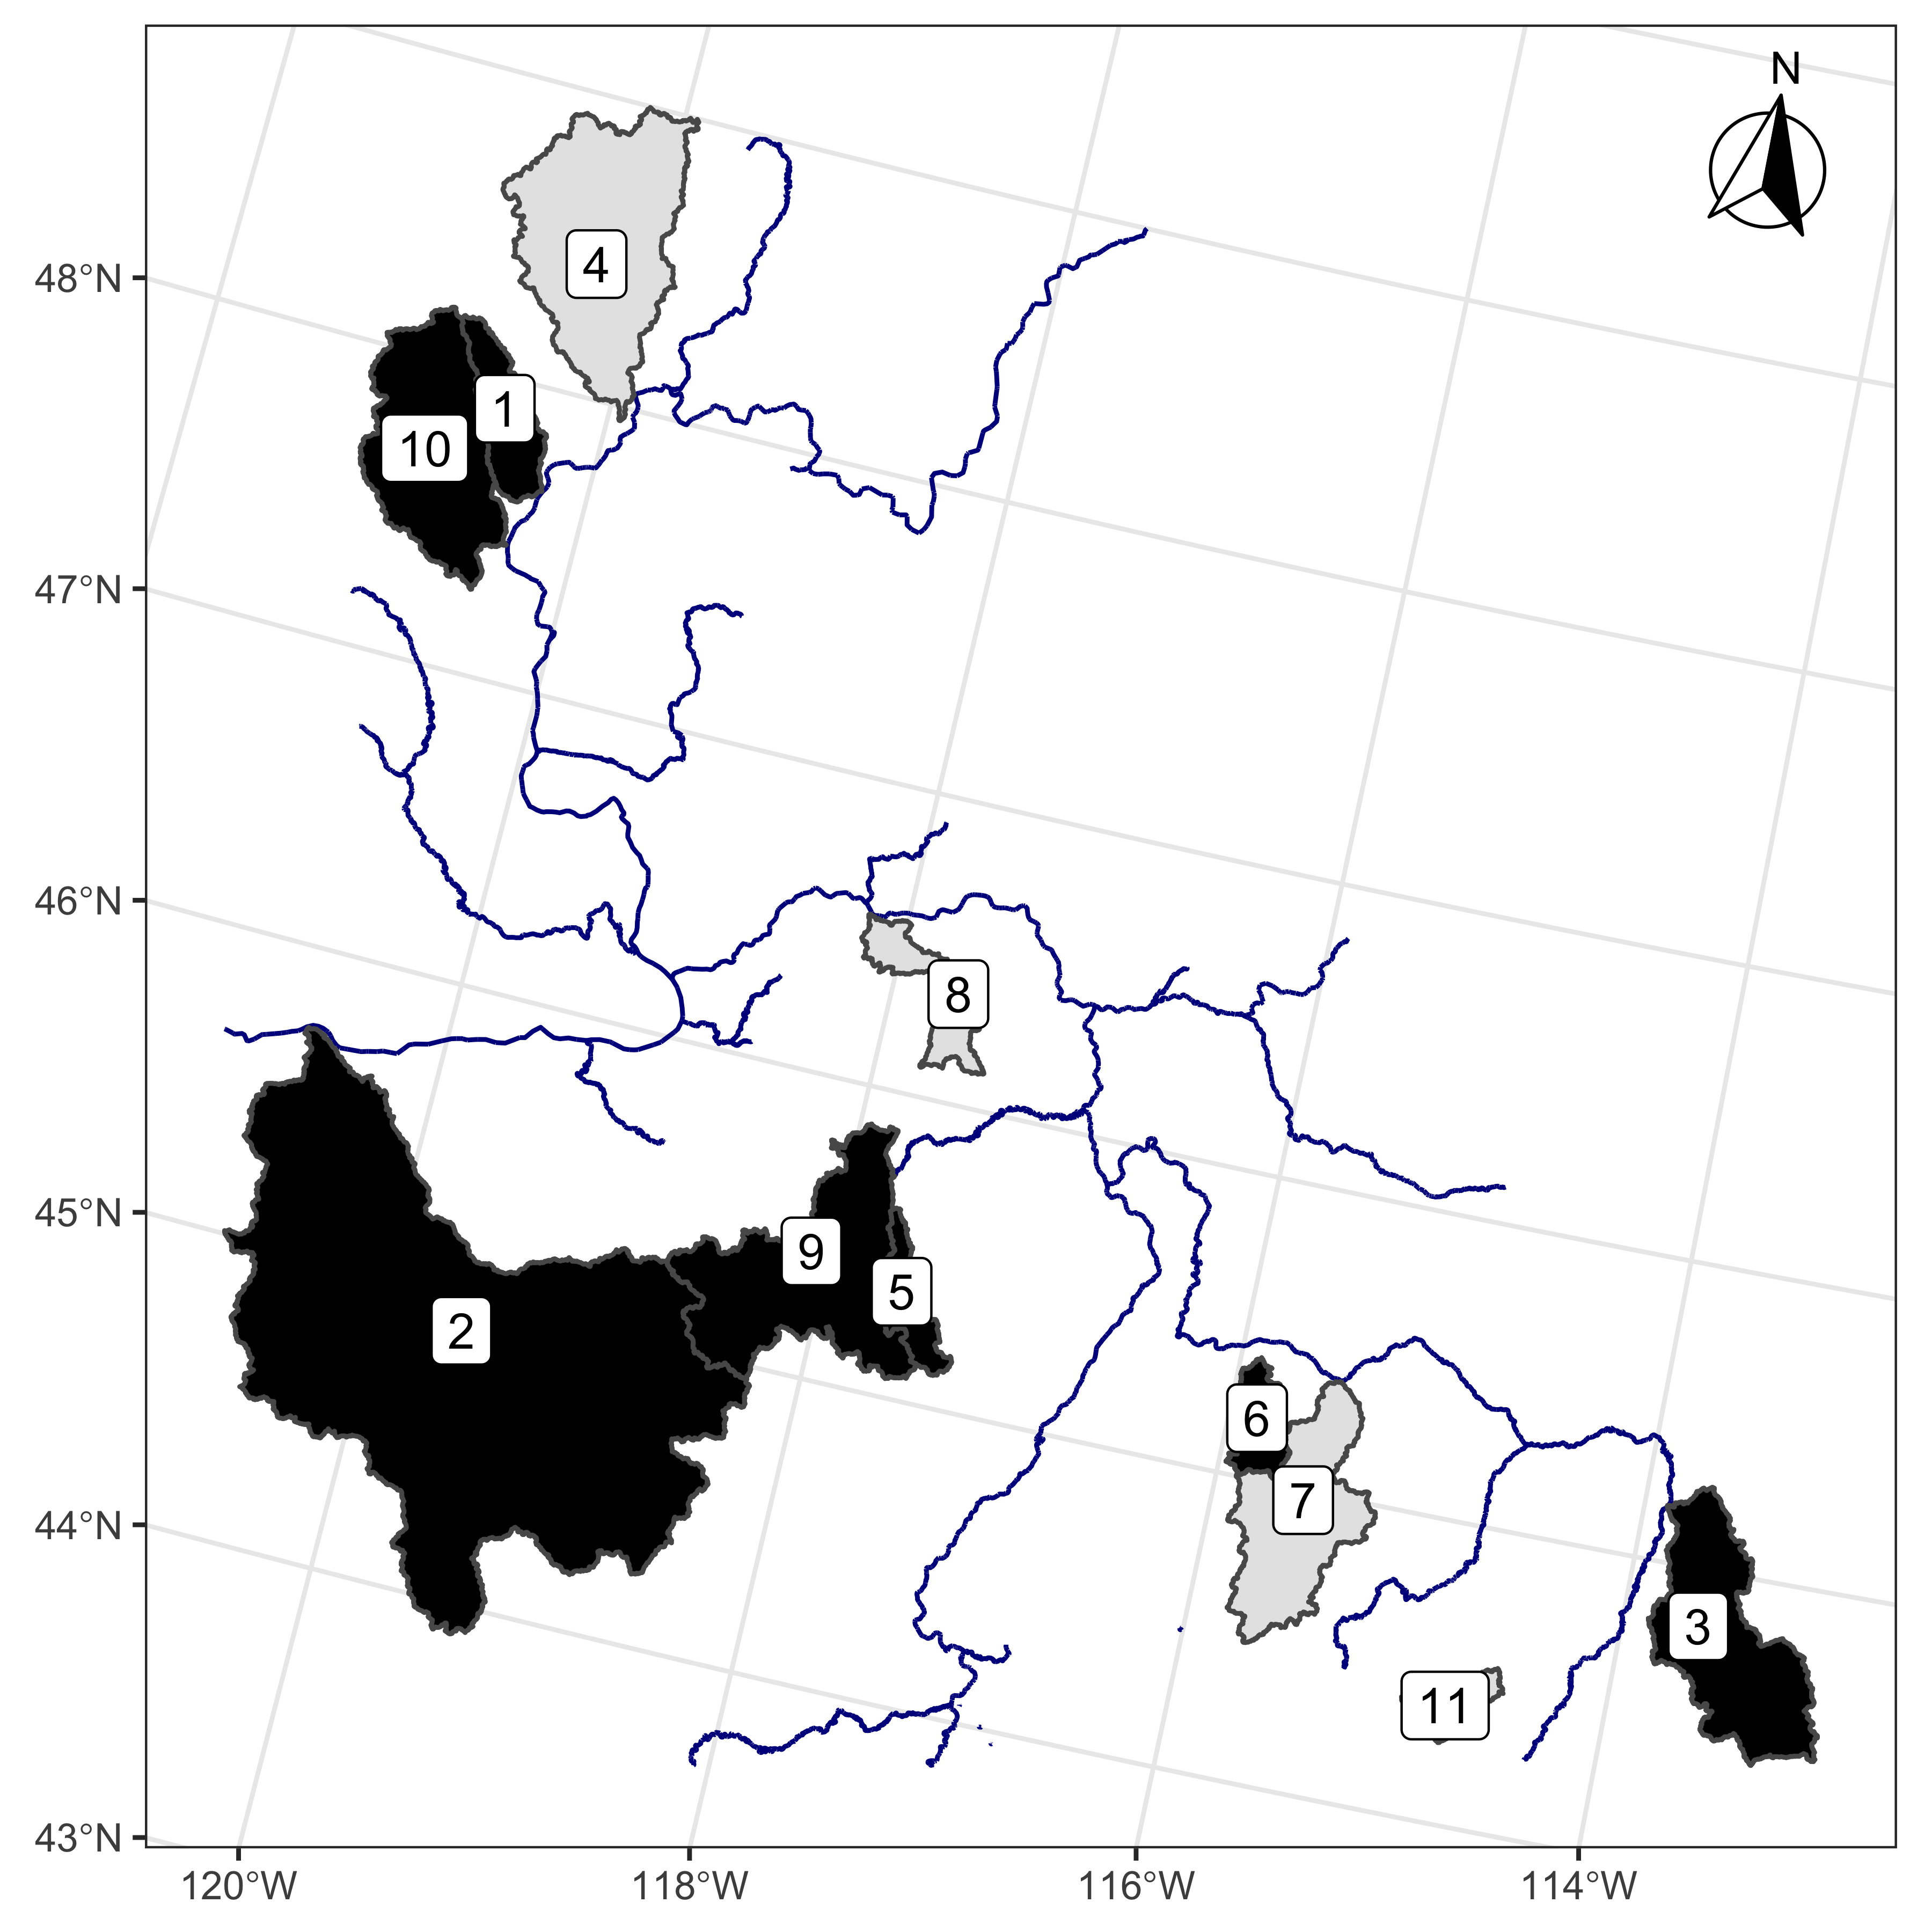
\includegraphics[width=0.85\linewidth]{../figures/ChampWtds} \caption{Watersheds with CHaMP habitat data. Watersheds in black also contain paired fish data. Watershed names are: 1 - Entiat, 2 - John Day, 3 - Lemhi, 4 - Methow, 5 - Minam, 6 - Secesh, 7 - South Fork Salmon, 8 - Tucannon, 9 - Upper Grande Ronde, 10 - Wenatchee, 11 - Yankee Fork.}\label{fig:wtsd-map}
\end{figure}

\newpage

\begin{figure}
\includegraphics[width=1\linewidth]{../figures/QRF_flowchart} \caption{Conceptual diagram showing input data sources, modeling decisions, model outputs etc. for the QRF and extrapolation models.}\label{fig:model-diag}
\end{figure}

\newpage

\begin{figure}
\centering
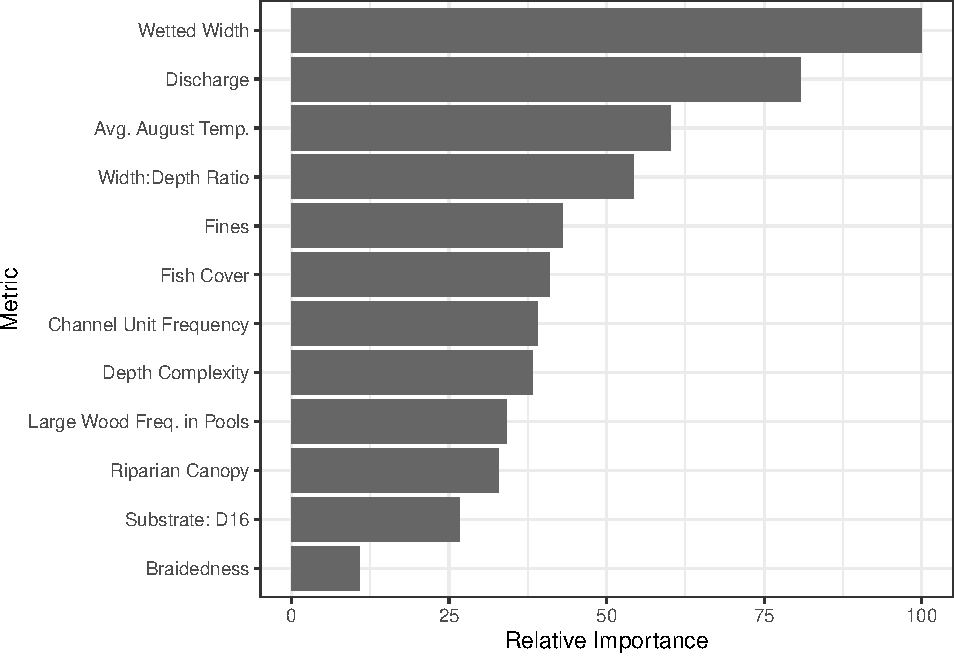
\includegraphics{../figures/rel-imp-figure-1.pdf}
\caption{\label{fig:rel-imp-figure}Relative importance of each habitat covariate included in the quantile random forest (QRF) model to predict habitat capacity, during summer months, for spring/summer-run Chinook salmon parr}
\end{figure}

\newpage

\begin{figure}
\centering
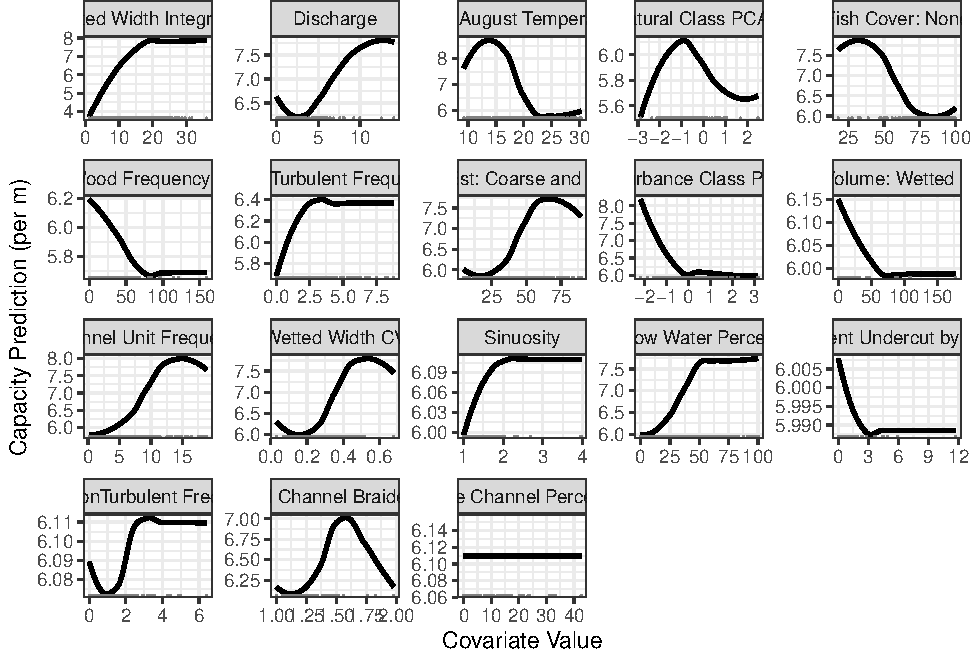
\includegraphics{../figures/pdp-figure-1.pdf}
\caption{\label{fig:pdp-figure}Partial dependence plots for the spring/summer-run Chinook salmon parr capacity quantile random forest (QRF) model, depicting how parr capacity shifts as each habitat metric changes, assuming all other habitat metrics remain at their mean values. Tick marks along the X-axis depict observed values.}
\end{figure}

\newpage

\begin{figure}
\centering
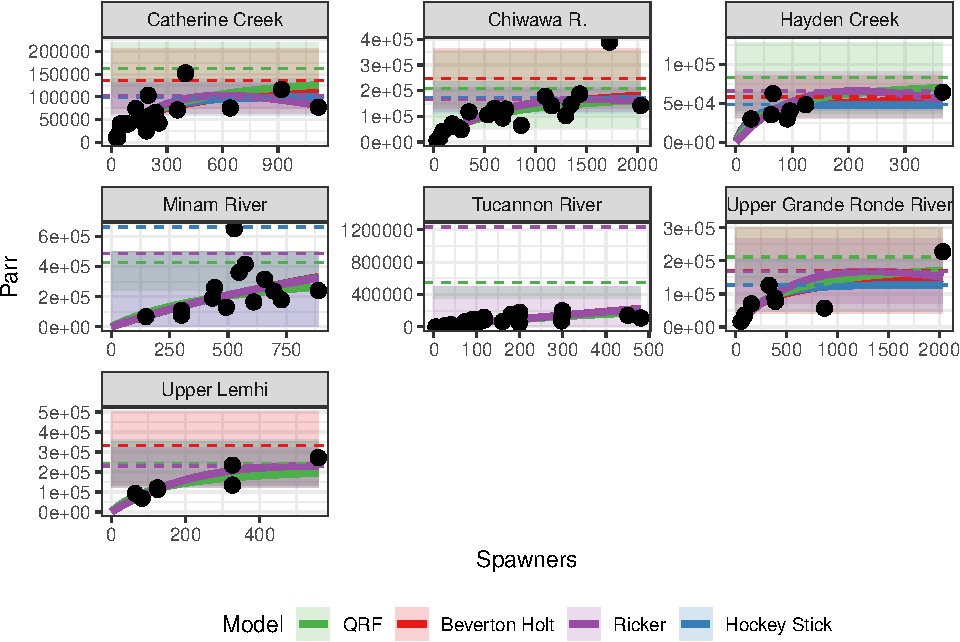
\includegraphics{../figures/sr-figure-1.pdf}
\caption{\label{fig:sr-figure}Spawner-recruit data from nine watersheds. Solid lines are the spawner-recruit curve, dashed lines are the estimated capacity, and shaded polygons depict the 95\% confidence intervals of capacity. Red corresponds to Beverton-Holt models, purple to Ricker models, blue to hockey stick models, and green to QRF estimates. The QRF solid curve is a Beverton-Holt model with the capacity parameter fixed to the QRF estimate of capacity. A few curves with high capacity estimates were not plotted to improve readability.}
\end{figure}

\end{document}
